\section{SpadesLogic}


\subsection{introduction}
	Spades is a trick-taking card game devised in the United States in the 1930s. It can be played as either a partnership or solo/"cutthroat" game. The object is to take at least the number of tricks (also known as "books") that were bid before play of the hand began. Spades is a descendant of the Whist family of card games, which also includes Bridge, Hearts, and Oh Hell. Its major difference as compared to other Whist variants is that, instead of trump being decided by the highest bidder or at random, the Spade suit is always trumps, hence the name. (Wikipedia)

\subsection{Rules}
	
\textbf{The Pack} \newline
The standard 52-card pack is used.\newline

\textbf{Rank of Suits} \newline
The spade suit is always trump.\newline

\textbf{Rank of Cards}\newline
A (high), K, Q, J, 10, 9, 8, 7, 6, 5, 4, 3, 2.\newline

\textbf{Object of the Game}\newline
To win at least the number of tricks bid.\newline

\textbf{The Deal} \newline
The first dealer is chosen by a draw for high card, and thereafter the turn to deal proceeds clockwise. The entire deck is dealt one at a time, face down, beginning on the dealer's left. The players then pick up their cards and arrange them by suits.
The Bidding

Each player decides how many tricks he will be able to take. The player to the dealer's left starts the bidding and, in turn, each player states how many tricks he expects to win. There is only one round of bidding, and the minimum bid is One. Every player must make a bid; no player may pass. No suit is named in the bid, for as the name of the game implies, spades are always trump.\newline

\textbf{The Play}\newline
The game is scored by hands, and the winner must make a certain number of points, which is decided before the game begins. Five hundred points is common, but 200 points is suitable for a short game. The player on the dealer's left makes the opening lead, and players must follow suit, if possible. If a player cannot follow suit, he may play a trump or discard. The trick is won by the player who plays the highest trump or if no trump was played, the player who played the highest card in the suit led. The player who wins the trick leads next. Play continues until none of the players have any cards left. Each hand is worth 13 tricks. Spades cannot be led unless played previously or player to lead has nothing but Spades in his hand.
How to Keep Score

For making the contract (the number of tricks bid), the player scores 10 points for each trick bid, plus 1 point for each overtrick.

For example, if the player's bid is Seven and he makes seven tricks, the score would be 70. If the bid was Five and the player won eight tricks, the score would be 53 points: 50 points for the bid, and 3 points for the three overtricks. In some games, overtricks are called "bags" and a deduction of 100 points is made every time a player accumulates 10 bags. Thus, the object is always to fulfill the bid exactly.

If the player "breaks contract," that is, if he takes fewer than the number of tricks bid, the score is 0. For example, if a player bids Four and wins only three tricks, no points are awarded.
One of the players is the scorer and writes the bids down, so that during the play and for the scoring afterward, this information will be available to all the players. When a hand is over, the scores should be recorded next to the bids, and a running score should be kept so that players can readily see each other's total points. If there is a tie, then all players participate in one more round of play. (bicyclecards.com)

\subsection{Logic}

As we are dealing with a \textbf{thin client | fat server} model, figure 1 outlines the general idea behind communication required for the game of Spades. The client will initialize the process with a login request. After which \textit{(assuming success)} the server will reply and grant the client access to the game lobby. The client will either attempt to join a game or instantiate a new one. After the game is fully set up the game initializes a loop handing the client - server for the remainder of the game. The server sends the state of the game along with a list of legal moves. The client will reply. This process will continue until the game is either interrupted or completed. After which, the server grants access to the lobby.  	

\begin{figure}
		% Center the figure.
		\begin{center}
		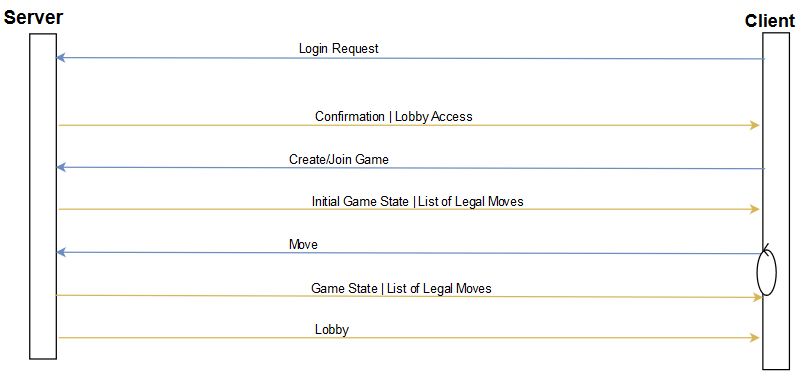
\includegraphics{graphics/SLfigure1}
		% Create a subtitle for the figure.
		\caption{Server - Client model for spades.}
		% Define the label of the figure. It's good to use 'fig:title', so you know that the label belongs to a figure.
		\label{Figure 1}
		\end{center}
	\end{figure}
	
	\begin{figure}
		% Center the figure.
		\begin{center}
		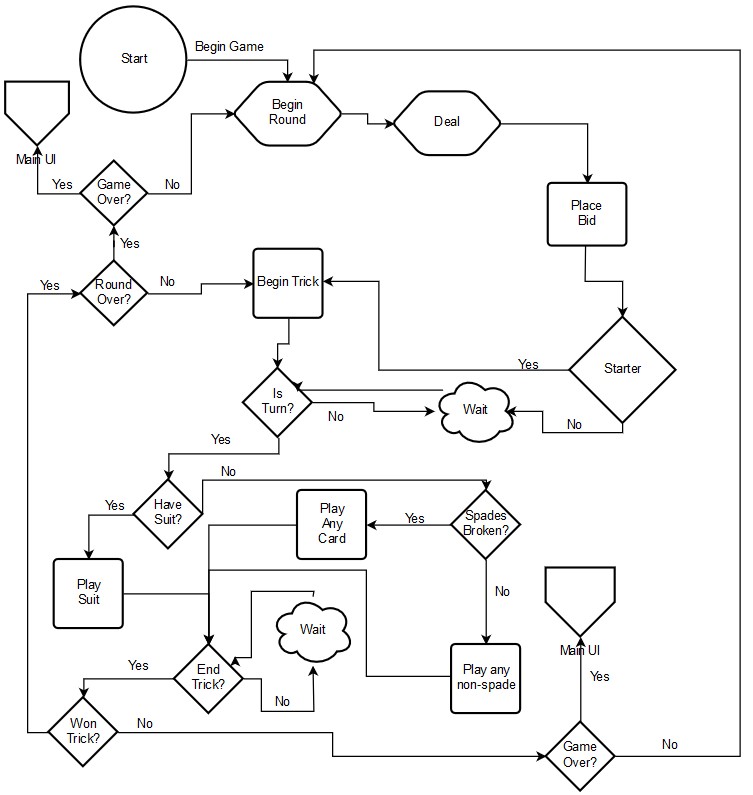
\includegraphics{graphics/SLfigure2}
		% Create a subtitle for the figure.
		\caption{Activity diagram for spades.}
		% Define the label of the figure. It's good to use 'fig:title', so you know that the label belongs to a figure.
		\label{Figure 1}
		\end{center}
	\end{figure}
	
